\achapter{14}{Continuity and Homeomorphisms}\label{chap:continuity_topology}


\vspace*{-17 pt}
\framebox{
\parbox{\dimexpr\linewidth-3\fboxsep-3\fboxrule}
{\begin{fqs}
\item How do we define a continuous function between topological spaces?
\item What is the difference between metric equivalence and topological equivalence?
\item What is a homeomorphism? What does it mean for two topological spaces to be homeomorphic?
\item What is a topological invariant? Why are topological invariants useful?
\end{fqs}}}

\vspace*{13 pt}

\csection{Introduction}\label{sec_cont_top_intro}

Recall that we could characterize a function $f$ from a metric space $(X,d_X)$ to a metric space $(Y,d_Y)$ as continuous at $a \in X$ if $f^{-1}(N)$ is a neighborhood of $a$ in $X$ whenever $N$ is a neighborhood of $f(a)$ in $Y$. We have defined neighborhoods in topological spaces, so we can use this characterization as our definition of a continuous function from one topological space to another. 

\begin{definition} \label{def:Continuity_topology} A function $f$ from a topological space $(X, \tau_X)$ to a topological space $(Y, \tau_Y)$ is \textbf{continuous at a point}\index{continuity in a topological space} $a \in X$ if $f^{-1}(N)$ is a neighborhood of $a$ in $X$ whenever $N$ is a neighborhood of $f(a)$ in $Y$. The function $f$ is \textbf{continuous} if $f$ is continuous at each point in $X$.
\end{definition}

We saw that in metric spaces, a useful characterization of continuity was in terms of open sets. It is not surprising that we have the same characterization in topological spaces. You may assume the result of Theorem \ref{thm:PA_TS_Open_continuity} (the topological space version of Theorem \ref{thm:Open_continuity} on \pageref{thm:Open_continuity} for metric spaces) for this activity. 

\begin{theorem} \label{thm:PA_TS_Open_continuity} Let $f$ be a function from a topological space $(X,\tau_X)$ to a topological space $(Y,\tau_Y)$. Then $f$ is continuous if and only if $f^{-1}(O)$ is an open set in $X$ whenever $O$ is an open set in $Y$.  
\end{theorem}

\begin{pa}  ~
\be
\item Let 
\[(X, \tau_X) = (\{1,2,3,4\}, \{\emptyset, \{1\}, \{2\}, \{1,2\}, X \})\]
and let 
\[(Y, \tau_Y) = (\{2,4,6,8\}, \{\emptyset, \{4\}, \{6\}, \{4,6\}, Y\}).\]
Define $f: X \to Y$ by $f(x) = 2x$. 
	\ba
	\item Is $f$ continuous at $4$?

	\item Is $f$ a continuous function? 

	\ea

\item Let 
\[(X, \tau_X) = (\{1,2,3,4\}, \{\emptyset, \{1\}, \{2\}, \{1,2\}, \{3,4\}, X \})\]
and let 
\[(Y, \tau_Y) = (\{a,b,c\}, \{\emptyset, \{a\}, \{a,c\}, Y\}).\] 
Define $f: X \to Y$ by $f(1) = a$, $f(2) = c$, $f(3) = f(4) = b$. 
	\ba
	\item Show that $f$ is a continuous function.

	\item Even though $f$ is continuous, it is possible that $f(O)$ may not be open for every open set in $X$. Find such an example for this function $f$. 
	
	\ea
	
Functions $f$ that have the property that $f(O)$ is open whenever $O$ is open in $X$ are called \emph{open} functions.

\begin{definition} Let $f: X \to Y$ be a function from a topological space $X$ to a topological space $Y$. Then $f$ is an \textbf{open} function\index{function!open}\index{open function} if $f(U)$ is open in $Y$ whenever $U$ is open in $X$. 
\end{definition}

There is a similar definition of a \emph{closed} function. 
	
	\item Let $X= \{1,2,3,4,5\}$ and $\tau = \{\emptyset,\{1\}, \{3,5\}, \{1,3,5\}, X\}$. Define $f: X \to X$ by $f(x) = \la x-3 \ra+1$. At which points is $f$ continuous? Is $f$ a continuous function?
	
\item Let $f:(\Z,\tau_{FC}) \to (\Z, d_E)$ where $f(n) = n$ and $\tau_{FC}$ is the finite complement topology. Is $f$ a continuous function? If $f$ is not continuous, exhibit a specific point at which $f$ fails to be continuous. Explain.

\item Let $f:(\Z, d_E) \to (\Z,\tau_{FC})$ where $f(n) = n$ and $\tau_{FC}$ is the finite complement topology. Is $f$ a continuous function? If $f$ is not continuous, exhibit a specific point at which $f$ fails to be continuous. Explain. 

\item It can sometimes be easier to show that a function $f$ mapping a topological space $(X,d_X)$ to a topological space $(Y,d_Y)$ is continuous by working with a basis instead of all open sets. Let $\B$ be a basis for the topology on $Y$. Is it the case that if $f^{-1}(B)$ is open for every $B \in \B$, then $f$ is continuous? Verify your result. 

\ee

\end{pa}

\begin{comment}

\ActivitySolution

\be
\item Let 
\[(X, \tau_X) = (\{1,2,3,4\}, \{\emptyset, \{1\}, \{2\}, \{1,2\}, X \}) \text{ and } (Y, \tau_Y) = (\{2,4,6,8\}, \{\emptyset, \{4\}, \{6\}, \{4,6\}, Y\}).\]
Define $f: X \to Y$ by $f(x) = 2x$. 
	\ba
	\item  Any neighborhood of $f(4)=8$ will have to contain an open set that contains $8$. The only open set in $Y$ that contains $8$ $Y$. Now $f^{-1}(Y) = X$ is an open set that contains $4$. So $f^{-1}(N)$ is a neighborhood of $4$ in $X$ whenever $N$ is a neighborhood of $8$ in $Y$. We conclude that $f$ is continuous at $4$.

	\item Note that $\{6\}$ is an open set in $Y$, but $f^{-1}(\{6\}) = \{3\}$ is not an open set in $X$. Therefore, $f$ is not a continuous function. 
	
	\ea

\item 
	\ba
	\item We determine $f^{-1}(O)$ for every open set $O$ in $Y$:
	\begin{itemize}
\item $f^{-1}(\emptyset) = \emptyset$
\item $f^{-1}(\{a\}) = \{1\}$
\item $f^{-1}(\{a,c\}) = \{1,2\}$
\item $f^{-1}(Y) = X$.
\end{itemize}
Since $f^{-1}(O)$ is open in $X$ for every open set $O$ in $Y$, then $f$ is a continuous function. 

	\item Notice that $f(\{3,4\}) = \{b\}$, which is not open in $Y$, so $f$ is not an open function.
	
	\ea
	
\item  First note that $f(1)=f(5)=3$, $f(2)=f(4)=2$, and $f(3) = 1$. So the inverse images of the open sets in $X$ are 
\begin{itemize}
\item $f^{-1}(\emptyset) = \emptyset$
\item $f^{-1}(\{1\}) = \{3\}$
\item $f^{-1}(\{3,5\}) = \{1,5\}$
\item $f^{-1}(\{1,3,5\}) = \{1,3,5\}$
\item $f^{-1}(X) = X$
\end{itemize}

Since $f^{-1}(\{3,5\})$ is not an open set in $X$, we see that $f$ is not a continuous function. We examine each point in turn to determine the continuity of $f$ at the points in $X$.
\begin{itemize}
\item Any neighborhood of $f(1)$ must contain one of the sets $\{3,5\}$, $\{1,3,5\}$ or $X$. The inverse images of each of these sets contains the neighborhood $\{1\}$ of $1$. So $f$ is continuous at $1$. 
\item The only neighborhood of $f(2)$ is $X$, so $f$ is continuous at $2$.
\item The open set $\{1\}$ is a neighborhood of $f(3)$, but $f^{-1}(\{1\})$ does not contain any open set that contains $3$. So $f$ is not continuous at $3$. 
\item The only neighborhood of $f(4)$ is $X$, so $f$ is continuous at $4$.
\item The open set $\{3,5\}$ is a neighborhood of $f(5)$, but $f^{-1}(\{3,5\})$ does not contain any open set that contains $5$. So $f$ is not continuous at $5$.
\end{itemize}

\item  The function $f$ is not continuous. The topology on $\Z$ induced by the Euclidean metric is the discrete topology. So the set $\{1\}$ is an open subset of $(\Z, d_E)$. However, $f^{-1}(\{1\}) = \{1\}$ is a set in $\Z$ whose compliment is infinite. So $f^{-1}(\{1\})$ doesn't contain a neighborhood of $1$ and $f$ is not continuous at $1$. We conclude that $f$ is not continuous. The same argument shows that $f$ isn't continuous at any point in $(\Z, \tau_{FC})$.  


\item  The topology on $\Z$ induced by the Euclidean metric is the discrete topology, so any subset of $(\Z, d_E)$ is open. Thus, $f^{-1}(O)$ is open for any open subset $O$ of $(\Z, \tau_{FC})$. Therefore, $f$ is a continuous function. 


\item Let $O$ be an open set in $Y$. Then $O = \cup_{\alpha \in I} B_{\alpha}$, where $B_{\alpha} \in \B$ for all $\alpha$ in some indexing set $I$. We know that 
\[f^{-1}(O) = \bigcup_{\alpha \in I} f^{-1}(B)_{\alpha}.\]
Since each $f^{-1}(B)_{\alpha}$ is open in $X$, it follows that $f^{-1}(O)$ is open in $X$. Thus, $f$ is continuous. 

\ee

\end{comment}

To complete the introduction to this section, we prove Theorem \ref{thm:PA_TS_Open_continuity}. We prove one direction now and leave the other for the next activity. 

Let $f$ be a function from a topological space $(X, \tau_X)$ to a topological space $(Y, \tau_Y)$. We first assume that $f$ is continuous and show that $f^{-1}(O)$ is an open set in $X$ whenever $O$ is an open set in $Y$. Suppose that $O$ is an open set in $Y$. To show that $f^{-1}O)$ is open in $X$, we will show that $f^{-1}(O)$ is a neighborhood of each of its points. Let $a \in f^{-1}(O)$. Then $f(a) \in O$. Since $O$ is an open set, $O$ is a neighborhood of $f(a)$. The fact that $f$ is continuous means that $f^{-1}(O)$ is a neighborhood of $a$. So $f^{-1}(O)$ is a neighborhood of each of its points and $f^{-1}(O)$ is an open set.

\begin{activity} Now we prove the remaining implication in Theorem \ref{thm:PA_TS_Open_continuity}. That is, let $f$ be a function from a topological space $(X, \tau_X)$ to a topological space $(Y, \tau_Y)$, and assume that $f^{-1}(O)$ is open whenever $O$ is open in $Y$. We will prove that $f$ is a continuous function.

\ba

\item Using the definition, what does it take to show that $f$ is a continuous function?

\item Let $a \in X$ and suppose that $N$ is a neighborhood of $f(a)$ in $Y$. What can we conclude from $N$ being a neighborhood?

\item Use the assumption about $f$ in this activity to explain why $f^{-1}(N)$ is a neighborhood of $a$ in $X$. 

\item Explain how we have shown that $f$ is a continuous function.

\ea

\end{activity}

\begin{comment}

\ActivitySolution

\ba

\item To show that $f$ is continuous we will prove that $f^{-1}(N)$ is a neighborhood of $a \in X$ whenever $N$ is a neighborhood of $f(a)$ in $Y$. 

\item Let $a \in X$ and let $N$ be a neighborhood of $f(a)$ in $Y$. Then $N$ contains an open set $O$ with $f(a) \in O$. 

\item By our hypothesis, we can conclude that $f^{-1}(O)$ is open in $X$. But if $x \in f^{-1}(O)$, then $f(x) \in O \subseteq N$. So $f^{-1}(O) \subseteq f^{-1}(N)$ and so $f^{-1}(N)$ is a neighborhood of $a$ in $X$. 

\item Since $a$ was chosen arbitrarily in $X$, we can conclude that $f^{-1}(N)$ is a neighborhood of $a$ in $X$ whenever $N$ is a neighborhood of $f(a)$ in $Y$. Therefore, $f$ is a continuous function.

\ea

\end{comment}

The following theorem is the topological analog of Theorem \ref{thm:closed_sets_continuity_MS} on page \pageref{thm:closed_sets_continuity_MS}. The proof is left for Exercise (\ref{ex:closed_sets_continuity_TS}).

\begin{theorem} \label{thm:closed_sets_continuity_TS} Let $f$ be a function from a topological space $(X,\tau_X)$ to a topologicval space $(Y,\tau_Y)$. Then $f$ is continuous if and only if $f^{-1}(C)$ is closed in $X$ whenever $C$ is a closed set in $Y$.  
\end{theorem}

\csection{Metric Equivalence}\label{sec_metric_equiv}

We have seen that we can make a set into a metric space with different metrics. For example, the spaces $(\R^2, d_E)$, $(\R^2, d_T)$, $(\R^2, d_M)$, and $(\R^2, d)$ are all metric spaces, where $d_E$ is the Euclidean metric, $d_T$ the taxicab metric, $d_M$ the max metric, and $d$ the discrete metric. But are these metric spaces really ``different" metric spaces? What do we mean by ``different"? 

\begin{activity} We might consider two metric spaces $(X, d_X)$ and $(Y, d_Y)$ to be equivalent if we can find a bijection between the two sets $X$ and $Y$ that preserves the metric properties. That is, find a bijective function $f : X \to Y$ such that $d_X(a,b) = d_Y(f(a), f(b))$ for all $a,b \in X$. In other words, $f$ preserves distances. 
	\ba
	\item Let $X = ((0,1), d_X)$ and $Y = ((0,2), d_Y)$, with both $d_X$ and $d_Y$ the Euclidean metric. Is it possible to find a bijection $f : X \to Y$ that preserves the metric properties? Explain. 
	
\item Now let $X = ((0,1), d_X)$ and $Y = ((0,2), d_Y)$, where $d_X$ is defined by $d_X(a,b) = 2 | a-b |$ and $d_Y = d_E$. You may assume that $d_X$ is a metric. Is it possible to find a bijection $f : X \to Y$ that preserves the metric properties? Explain. 

	\ea

\end{activity}

\begin{comment}

\ActivitySolution
	\ba
	\item The answer is no. Suppose to the contrary that there is a bijective function $f: (0,1) \to (0,2)$ so that 
\[d_X(a,b) = d_Y(f(a), f(b))\]
for all $a,b \in X$. Let $u, v \in Y$. The surjectivity of $f$ implies that there exists $a,b \in X$ such that $f(a) = u$ and $f(b) = v$. Then
\[| u - v | = | f(a) - f(b) | = | a-b| \leq 1.\]
So $| u-v | \leq 1$ for all $u, v \in Y$. But $1.75$ and $0.25$ are in $Y$ and 
\[| 1.75-0.25 | = 1.5 > 1.\]
So no such function can exist. 


\item  The answer is yes. Let $f:X \to Y$ be defined by $f(x) = 2x$. We will show that $f$ is an injection. Let $a_1, a_2 \in X$ and assume $f(a_1) = f(a_2)$. Then $2a_1 = 2a_2$ from which it follows that $a_1 = a_2$. So $f$ is an injection. Let $y \in Y$. Then $0 < y < 2$. So $0 < \frac{y}{2} < 1$ and $\frac{y}{2} \in X$. Since 
\[f\left(\frac{y}{2}\right) = 2\left(\frac{y}{2}\right) = y,\]
we see that $f$ is a surjection. Thus, $f$ is a bijection. 

Finally, let $a, b \in X$. Then
\[d_Y(f(a),f(b)) = | 2a-2b | = 2| a-b | = d_X(a,b).\]
So $f$ preserves distances. 

	\ea


\end{comment}

If there is a bijection between metric spaces that preserves distances, we say that the metric spaces are \emph{metrically equivalent}.  

\begin{definition} \label{def:MS_metric_equivalence} Two metric spaces $(X,d_X)$ and $(Y,d_Y)$ are \textbf{metrically equivalent}\index{metrically equivalent} if there is a bijection $f : X \to Y$ such that 
\[d_X(x,y) = d_Y(f(x),f(y))\]
for all $x,y \in X$. 
\end{definition}

Because $f$ is a bijection, it will also be the case in Definition \ref{def:MS_metric_equivalence} that 
\[d_Y(u,v) = d_X(f^{-1}(u), f^{-1}(v))\]
for all $u$ and $v$ in $Y$. The proof is left for Exercise (\ref{ex:isometry_reverse}). 
%Let $u,v$ be elements in $Y$. Since $f$ is a bijection, there exist $x$ and $y$ in $X$ such that $f(x) = u$ and $f(y) = b$, or $u = f^{-1}(x)$ and $b = f^{-1}(y)$. Then
%\[d_Y(u,v) = d_Y(f(x),f(y)) = d_X(x,y) = d_X(f^{-1}(u), f^{-1}(v)).\]

Any function $f$ that preserves distances (like the one in Definition \ref{def:MS_metric_equivalence}) is called an \emph{isometry}. 

\begin{definition} A function $f$ from a metric space $(X,d_X)$ to a metric space $(Y, d_Y)$ is an \textbf{isometry}\index{isometry} if $f$ is a bijection and 
\begin{equation} \label{eq:distance_preserving} 
d_Y(f(a),f(b)) = d_X(a,b)
\end{equation}
for all $a, b \in X$. 
\end{definition}

Metric equivalence is a very strong type of equivalence -- the existence of an isometry does not allow for much flexibility since distances must be preserved. From a topological perspective, we are only concerned about the open sets -- there are no distances. The open unit ball in $(\R^2, d_E)$ and the open ball in $(\R^2, d_M)$ (where $d_E$ is the Euclidean metric and $d_M$ is the max metric) are not that different as we can see in Figure \ref{F:Equivalence}. If we don't worry about preserving distances, we can stretch the open ball $B_E = B((0,0),1)$ in $(\R^2, d_E)$ along the lines $y=x$ and $y=-x$ uniformly in a way to mold it onto the unit ball $B_M = B((0,0),1)$ in $(\R^2, d_M)$. The important thing is that this stretching will preserve the open sets. This is a much more forgiving type of equivalence and maintains the central idea of topology that we have discussed -- what properties of a space are not altered by stretching and bending the space. This type of equivalence that allows us to manipulate a space without fundamentally changing the open sets is called \emph{topological equivalence}. 
\begin{figure}[ht]
\begin{center}
\resizebox{!}{1.5in}{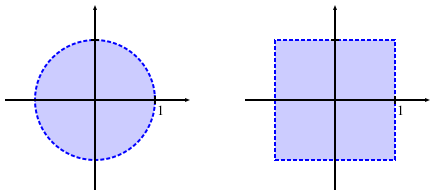
\includegraphics{Equivalence.eps}}
\caption{The open unit balls in $(\R^2, d_E)$ and $(\R^2, d_M)$.}
\label{F:Equivalence}
\end{center}
\end{figure}


\csection{Topological Equivalence}\label{sec_top_equiv}
 
When we can deform one set into another without poking holes in the set, we consider the two sets to be equivalent from a topological perspective. Such a deformation $f$ has to be a bijection to ensure that the two sets contain the same number of elements, continuous so that the inverse images of open sets are open, and $f^{-1}$ must be continuous so images of open sets are open. Such a function provides a one-to-one correspondence between open sets in the two spaces. This leads to the next definition.

\begin{definition} \label{def:MS_topological_equivalence} Two topological spaces $(X,d_X)$ and $(Y,d_Y)$ are \textbf{topologically equivalent}\index{topologically equivalent} if there is a continuous bijection $f : X \to Y$ such that $f^{-1}$ is also continuous.  
\end{definition}

Metric equivalence always implies topological equivalence (using the metric topologies), which is left for Exercise (\ref{ex:me_implies_te}). So metric equivalence is a stronger condition than topological equivalence.

The function $f$ (or $f^{-1}$) in Definition \ref{def:MS_topological_equivalence} is called a \emph{homeomorphism}.

\begin{definition} \label{def:Homeomorphism} Let $(X,\tau_X)$ and $(Y,\tau_Y)$ be topological spaces. A function $f: X \to Y$ is a \textbf{homeomorphism}\index{homeomorphism} if $f$ is a continuous bijection such that $f^{-1}$ is also continuous.  
\end{definition}

If there is a homeomorphism from $(X,\tau_X)$ to $(Y,\tau_Y)$ we say that the spaces $(X,\tau_X)$ to $(Y,\tau_Y)$ are \emph{homeomorphic}\index{homeomorphic spaces} topological spaces. 

It can be difficult to show directly that two metric spaces are homeomorphic, but there are ways to make the process easier in metric spaces. If $f$ is a homeomorphism from the metric space $(\R^2, d_E)$ to the metric space $(\R^2, d_M)$, the continuity of $f$ ensures a smooth deformation from $\R^2$ to $\R^2$. In terms of the metrics, this means that distances cannot get distorted too much -- in fact, the amount distances are distorted should be bounded. In other words, we might expect that there is a constant $K$ so that $d_E(x,y) \leq K d_M(f(x), f(y))$ for any $x, y \in \R^2$. The next theorem tells us that this is a sufficient condition for topological equivalence when we work in the same underlying space. 

\begin{theorem} Let $X$ be a set on which two metrics $d$ and $d'$ are defined. If there exist positive constants $K$ and $K'$ so that 
\begin{align*}
d'(x,y) &\leq K d(x,y) \\
d(x,y) &\leq K' d'(x,y)
\end{align*}
for all $x,y \in X$, then $(X,d)$ is topologically equivalent to $(X,d')$.  
\end{theorem}

\begin{proof} Let $X$ be a set on which two metrics $d$ and $d'$ are defined. Suppose there exist positive constants $K$ and $K'$ so that 
\begin{align*}
d'(x,y) &\leq K d(x,y) \\
d(x,y) &\leq K' d'(x,y)
\end{align*}
for all $x,y \in X$. Let $i_X : (X,d) \to (X,d')$ be the identity mapping. That is, $i_X(x)=x$ for all $x \in X$. We will prove that $i_X$ is a homeomorphism. We know that $i_X$ is a bijection, so we only need verify that $i_X$ and $i_X^{-1}$ are continuous. Let $\epsilon > 0$ be given, and let $a \in X$. Let $\delta = \frac{\epsilon}{K}$. Suppose $x \in X$ so that $d(x,a) < \delta$. Then 
\[d'(i_X(x), i_X(a)) = d'(x,a) \leq Kd(x,a) < K\delta = K\left(\frac{\epsilon}{K}\right) = \epsilon.\]
Thus, $i_X$ is continuous. The same argument shows that $i_X^{-1}$ is also continuous. Therefore, $i_X$ is a homeomorphism between $(X,d)$ and $(X,d')$. 
\end{proof}


\begin{activity} ~
\ba
\item Are $(\R^2,d_T)$ and $(\R^2, d_M)$ topologically equivalent? Explain.

\item Are $(\R^2,d_E)$ and $(\R^2, d_T)$ topologically equivalent? Explain.

\item Do you expect that $(\R^2,d_E)$ and $(\R^2, d_M)$ are topologically equivalent. Explain without doing any calculations or comparisons.

\ea

\end{activity}

\begin{comment}

\ActivitySolution

\ba
\item Let $x = (x_1,x_2)$ and $y=(y_1,y_2)$ be in $\R^2$. Notice that 
\[d_M(x,y) = \max\{| x_1-y_1 |, | x_2-y_2 |\} \leq | x_1-y_1 | + | x_2-y_2 | = d_T(x,y).\]
Also,
\[d_T(x,y) = | x_1-y_1 | + | x_2-y_2 | \leq 2\max\{| x_1-y_1 |, | x_2-y_2 |\} = 2d_M(x,y).\]
So $(\R^2,d_T)$ and $(\R^2, d_M)$ are topologically equivalent. 

\item Let $x = (x_1,x_2)$ and $y=(y_1,y_2)$ be in $\R^2$. Notice that 
\[d_E(x,y) = \sqrt{(x_1-y_1)^2 + (x_2-y_2)^2} \leq \sqrt{(x_1-y_1)^2} + \sqrt{(x_2-y_2)^2} =  | x_1-y_1 | + | x_2-y_2 | \leq d_T(x,y).\]
Also,
\[d_T(x,y) = | x_1-y_1 | + | x_2-y_2 | = \sqrt{(x_1-y_1)^2} + \sqrt{(x_2-y_2)^2} \leq \sqrt{(x_1-y_1)^2+(x_2-y_2)^2} + \sqrt{(x_1-y_1)^2+(x_2-y_2)^2} = 2d_E(x,y).\]
So $(\R^2,d_T)$ and $(\R^2, d_T)$ are topologically equivalent. 

\item If $f: (\R^2,d_T) \to (\R^2, d_M)$ and $g: (\R^2,d_E) \to (\R^2, d_T)$ are homeomorphisms, then we know that $f \circ g$ is a continuous bijection as is $(f \circ g)^{-1}$. So it must be the case that $(\R^2,d_E)$ and $(\R^2, d_M)$ are topologically equivalent. 
 
\ea

\end{comment}


\csection{Relations}\label{sec_relations}
We use the word ``equivalent" deliberately when talking about metric or topological equivalence. Recall that equivalence is a word used with relations, and that a relation is a way to compare two elements from a set. We are familiar with many relations on sets, ``$<$", ``$=$", ``$\geq$" on the integers, for example.  

\begin{definition} A \emph{relation}\index{relation} on a set $S$ is a subset $R$ of $S \times S$.
\end{definition}

For example, the subset $R = \{(a,a) \mid a \in \Z \}$ of $\Z \times \Z$ is the relation we call equals. If $R$ is a relation on a set $S$, we usually suppress the set notation and write $a \sim b$ if $(a,b) \in R$ and say that $a$ is related to $b$. In this case we often refer to $\sim$ as the relation instead of the set $R$. Sometimes we use familiar symbols for special relations. For example, we write $a = b$ if $(a,b) \in R = \{(a,a) \mid a \in \Z \}$.

When discussing relations, there are three specific properties that we consider.

\begin{itemize}
\item A relation $\sim$ on a set $S$ is \emph{reflexive} if $a \sim a$ for all $a \in S$.
\item A relation $\sim$ on a set $S$ is \emph{symmetric} if whenever $a \sim b$ in $S$ we also have $b \sim a$.
\item A relation $\sim$ on a set $S$ is \emph{transitive} if whenever $a \sim b$ and $b \sim c$ in $S$ we also have $a \sim c$.
\end{itemize}

When we use the word ``equivalence", we are referring to an equivalence relation.

\begin{definition} An \textbf{equivalence relation}\index{equivalence relation} is a relation on a set that is reflexive, symmetric, and transitive.  
\end{definition}


\begin{activity} ~
\ba
\item Explain why metric equivalence is an equivalence relation.

\item Explain why topological equivalence is an equivalence relation.

\ea

\end{activity}

\begin{comment}

\ActivitySolution

\ba
\item Let $(X, d_X)$, $(Y, d_Y)$, and $(Z, d_Z)$ be metric spaces. The identity function $id_X : X \to X$ is a bijection that satisfies 
\[d_X(x,y) = d_X(id_X(x), id_X(y)).\]
So $X$ is metrically equivalent to $X$ and metric equivalence is a reflexive relation. 

Suppose that there is a bijection $f: X \to Y$ such that 
\[d_X(x,y) = d_Y(f(x),f(y))\]
for all $x$ and $y$ in $X$. The fact that $f$ is a bijection means that $f^{-1}$ is a bijection from $Y$ to $X$. Let $u$ and $v$ be in $Y$. Then $x = f^{-1}(u)$ and $y = f^{-1}(v)$ are well defined in $X$. Then $f(x) = u$ and $f(y) = v$, and 
\[d_Y(u,v) = d_Y(f(x), f(y)) = d_X(x,y) = d_X(f^{-1}(u), f^{-1}(v)).\]
This makes $(Y, d_Y)$ metrically equivalent to $(X,d_X)$ and metric equivalence is a symmetric relation.

Finally, suppose that there is a bijection $f: X \to Y$ such that 
\[d_X(x,y) = d_Y(f(x),f(y))\]
for all $x$ and $y$ in $X$, and that there is a bijection $g: Y \to Z$ such that 
\[d_Y(u,v) = d_Z(g(u),g(v))\]
for all $u$ and $v$ in $Y$. Let $h = g \circ f$. We know that the composite of bijections is a bijection, so $h: X to Z$ is a bijection. Moreover, if $x$ and $y$ are in $X$, then 
\[d_X(x,y) = d_Y(f(x),f(y)) = d_Z(g(f(x)), g(f(y)) = d_Z(h(x), h(y)).\]
So $X$ is metrically equivalent to $Z$ and metric equivalence is a transitive relation. We conclude that metric equivalence is an equivalence relation. 

\item Let $(X, \tau_X)$, $(Y, \tau_Y)$, and $(Z, \tau_Z)$ be topological spaces. The identity function $id_X : X \to X$ is a continuous bijection whose inverse ($id_X$) is also a continuous bijection. So $X$ is topologically equivalent to $X$ and topological equivalence is a reflexive relation. 

Suppose that there is a continuous bijection $f: X \to Y$ such that $f^{-1}$ is also continuous. Then $f^{-1} : Y \to X$ is a continuous bijection whose inverse is also continuous. This makes $Y$ topologically equivalent to $X$ and topological equivalence is a symmetric relation.

Finally, suppose that there is a continuous bijection $f: X \to Y$ such that $f^{-1}$ is also continuous, and that there is a continuous bijection $g: Y \to Z$ such that $g^{-1}$ is also continuous. Let $h = g \circ f$. We know that the composite of bijections is a bijection, so $h: X to Z$ is a bijection. Moreover, the composite of continuous function is continuous. So $h$ is a continuous bijection from $X$ to $Z$ such that $h^{-1}$ is also continuous. Thus, 
So $X$ is topologically equivalent to $Z$ and topological equivalence is a transitive relation. We conclude that topological equivalence is an equivalence relation. 

\ea


\end{comment}

Equivalence relations are important because an equivalence relation on a set $S$ partitions the set into a disjoint union of equivalence classes. Since topological equivalence is an equivalence relation, we can treat the spaces that are topologically equivalent to each other as being essentially the same space from a topological perspective. Under the relation of homeomorphism we call the equivalence classes \emph{homeomorphism} classes. 


\csection{Topological Invariants}\label{sec_top_invar}
Homeomorphic topological spaces are essentially the same from a topological perspective, and they share many properties, but not all. The properties they share are called \textit{topological invariants} or \emph{topological properties}.

\begin{definition} A property of a topological space $X$ is a \textbf{topological property}\index{topological property} (or \textbf{topological invariant}\index{topological invariant}) if every topological space homeomorphic to $X$ has the same property. 
\end{definition}

\begin{activity} Which of the following are topological invariants? That is for topological spaces $(X, \tau_X)$ and $(Y, \tau_Y)$, if $X$ and $Y$ are homeomorphic space and $X$ has the property, does it follow that $Y$ must also have that property?
\ba
\item $X$ has the indiscrete topology
\item $X$ has the discrete topology
\item $X$ has the finite complement topology
\item $X$ contains the number 2
\item $X$ contains exactly 13 elements
\ea
\end{activity}


\begin{comment}

\ActivitySolution
\ba
\item If $O$ is an open set in $T$, then $f^{-1}(O)$ is open in $X$. This means that $f^{-1}(O)$ is either $\emptyset$ or $X$. It follows that $O$ is either $\emptyset$ or $O = Y$. Thus, having the indiscrete topology is a topological invariant. 

\item Since there is a homeomorphism $f$ from $X$ to $Y$, the image of any open set in $X$ is open in $Y$. The fact that $f$ is an injection means that $\{f(x) \mid x \in X\}$ runs over all single point sets in $Y$, and these sets must be open. So having the discrete topology is a topological property.

\item Let $f$ be a homeomorphism from $X$ to $Y$. Let $O$ be an open set in $Y$.  We know that $f^{-1}(Y \setminus O) = X \setminus f^{-1}(O)$. Since $X \setminus f^{-1}(O)$ is open, the set $X \setminus f^{-1}(O)$ is finite. So $f^{-1}(Y \setminus O)$ is finite. The fact that $f$ is an injection means that $Y \setminus (O)$ is finite.  So every open set $O$ in $Y$ satisfies $Y \setminus O$ is finite. Now we have to prove the converse.

Suppose $B$ is a subset of $Y$ such that $Y \setminus B$ is finite. Then $f^{-1}(Y \setminus B)$ is finite. This implies that $X \setminus f^{-1}(B)$ is finite and so $f^{-1}(B)$ is open in $X$. Since $f^{-1}$ is continuous and $f$ is a bijection, $f(f^{-1}(B)) = B$ is open in $Y$. So having the finite complement topology is a topological property.

\item Containing a specific element is not a topological property. For example, $X = \{1,2\}$ and $Y = \{a,b\}$, both with the discrete topology, are homeomorphic, but $2 \notin Y$. 

\item Since a homeomorphism $f$ is a bijection, the number of elements in a set is preserved under $f$. So the number of elements in a set is a topological invariant.
 
\ea

\end{comment}

\csection{Summary}\label{sec_cont_top_summ}
Important ideas that we discussed in this section include the following.
\begin{itemize}
\item A function $f$ from a topological space $X$ to a topological space $Y$ is continuous if $f^{-1}(O)$ is open in $X$ whenever $O$ is open in $Y$. 
\item Two metric spaces $(X,d_X)$ and $(Y,d_Y)$ are metrically equivalent if there is a bijection $f : X \to Y$ such that 
\begin{align*}
d_X(x,y) &= d_Y(f(x),f(y)) \\
d_Y(u,v) &= d_X(f^{-1}(u), f^{-1}(v))
\end{align*}
for all $x,y \in X$ and $u,v \in Y$. That is, $X$ and $Y$ are metrically equivalent if there is a isometry $f$ from $X$ to $Y$ such that $f^{-1}$ is also an isometry. Topological equivalence is a less stringent condition. Two topological spaces $X$ and $Y$ are topologically equivalent if there is a continuous function $f$ from $X$ to $Y$ such that $f^{-1}$ is also continuous. That is, $X$ and $Y$ are topologically equivalent if there is a homeomorphism between $X$ to $Y$. 
\item A homeomorphism between topological spaces $X$ and $Y$ is a continuous function $f$ from $X$ to $Y$ such that $f^{-1}$ is also continuous. Two topological spaces $X$ and $Y$ are homeomorphic if there is a homeomorphism $f : X \to Y$. 
\item A topological invariant is any property that topological space $X$ has that must also be a property of any topological space homeomorphic to $X$. We can sometimes use topological invariants to determine if two topological spaces are not homeomorphic.
\end{itemize}

\csection{Exercises}\label{sec_cont_top_exer}

\be

\item \label{ex:isometry_reverse} Let $(X,d_X)$ and $(Y,d_Y)$ be metrically equivalent metric spaces, and let $f:X \to Y$ be a bijection such that 
\[d_X(x,y) = d_Y(f(x),f(y))\]
for all $x,y \in X$. Prove that 
\[d_Y(u,v) = d_X(f^{-1}(u), f^{-1}(v))\]
for all $u$ and $v$ in $Y$. 

\begin{comment}

\ExerciseSolution Let $u,v$ be elements in $Y$. Since $f$ is a bijection, there exist $x$ and $y$ in $X$ such that $f(x) = u$ and $f(y) = b$, or $u = f^{-1}(x)$ and $b = f^{-1}(y)$. Then
\[d_Y(u,v) = d_Y(f(x),f(y)) = d_X(x,y) = d_X(f^{-1}(u), f^{-1}(v)).\]

\end{comment}

\item Let $(X, \tau_X)$ and $(Y, \tau_Y)$ be topological spaces, and let $f : X \to Y$ be a homeomorphism. Let $A$ be a subset of $X$.
\ba
\item If $x$ is a limit point of $A$, must $f(x)$ be a limit point of $f(A)$? Prove your answer.

\item If $x$ is an interior point of $A$, must $f(x)$ be an interior point of $f(A)$? Prove your answer.

\item If $x$ is a boundary point of $A$, must $f(x)$ be a boundary point of $f(A)$? Prove your answer.

\ea

\begin{comment}

\ExerciseSolution

\ba
\item Let $x$ be a limit point of $A$ and let $O$ be an open set containing $f(x)$ in $Y$. Since $f$ is continuous, we know that $f^{-1}(O)$ is an open set in $X$ that contains $x$. Thus, $f^{-1}(O)$ contains a point $a$ in $A$ different from $x$. Since $a \in f^{-1}(O)$ we know that $f(a) \in O$. Also, $a \in A$ implies that $f(a) \in f(A)$. The fact that $f$ is a bijection means that $f(a) \neq f(x)$. But then $O$ contains the element $f(a)$ in $f(A)$ that is different from $f(x)$, so $f(x)$ is a limit point of $f(A)$. 

\item Let $x$ be an interior point of $A$. Then there is an open set $O$ with $x \in O \subseteq A$. The fact that $f^{-1}$ is continuous means that $f(O)$ is an open subset of $Y$. Since $O \subseteq A$, we also have $f(x) \in f(O) \subseteq f(A)$. So $f(A)$ is a neighborhood of $f(x)$ and $f(x)$ is an interior point of $f(A)$. 

\item Let $x$ be a boundary point of $A$, and let $O$ be an open set that contains $f(x)$. Since $f$ is continuous, we know that $f^{-1}(O)$ is an open set in $X$ that contains $x$. Thus, $f^{-1}(O)$ contains a point $a$ in $A$ and a point $c$ in $X \setminus A$. Then $f(a) \in f(A)$ and $f(x) \in f(X \setminus A) = Y \setminus f(A)$. Thus, $f(x)$ is a boundary point of $f(A)$. 

\ea


\end{comment}

\item \label{ex:me_implies_te} Let $(X, d_X)$ and $(Y, d_Y)$ be metrically equivalent metric spaces. Show that $X$ and $Y$ are topologically equivalent using the metric topologies. 

\begin{comment}

\ExerciseSolution Let $f : X \to Y$ be a bijection such that $d_X(x,y) = d_Y(f(x),f(y))$ for all $x, y \in X$. To show that $f$ is continuous in the metric topology, we will show that the inverse of any open ball in $Y$ is an open set in $X$. Let $B_Y = B(z,\delta)$ be an open ball in $Y$. Let $B_X = f^{-1}(B_Y)$. We will show that $B_X = B(f^{-1}(z), \delta)$ in $X$, which will verify that the inverse image of $B_Y$ under $f$ is an open set in $X$. 

Let $x \in B_X$. Then $x = f^{-1}(t)$ for some $t \in B_Y$, or $t = f(x)$. It follows that 
\[d_X(x,f^{-1}(z)) = d_Y(f(x),f(f^{-1}(z))) = d_Y(t,z) < \delta.\]
Thus, $x \in B(f^{-1}(z), \delta)$ and $B_X \subseteq B(f^{-1}(z), \delta)$. 

Now let $x \in B(f^{-1}(z), \delta)$. Then $d_X(x, f^{-1}(z)) < \delta$. Let $t = f(x)$. It follows that 
\[d_Y(t,z) = d_X(f^{-1}(t), f^{-1}(z)) = d_X(x, f^{-1}(z)) < \delta.\]
Thus, $t \in B_Y$ and $x \in f^{-1}(B_Y)$ or $x \in B_X$.  This shows that $B(f^{-1}(z), \delta) \subseteq B_X$, which allows us to conclude that $B_X = B(f^{-1}(z), \delta)$. Therefore, $f$ is continuous. The same argument applied to $f^{-1}$ shows that $f^{-1}$ is also continuous. So $X$ and $Y$ are topologically equivalent. 

\end{comment}

\item \label{ex:closed_sets_continuity_TS} Prove theorem \ref{thm:closed_sets_continuity_TS} that if $(X,\tau_X)$ and $(Y, \tau_Y)$ are topological spaces, and $f: X \to Y$ is a function, then $f$ is continuous if and only if $f^{-1}(C)$ is a closed set in $X$ whenever $C$ is a closed set in $Y$. 

\begin{comment}

\ExerciseSolution Assume that $f$ is a continuous function, and let $C$ be a closed set in $Y$. Since $C$ is closed, we know that $Y \setminus C$ is open. The continuity of $f$ means that $f^{-1}(Y \setminus C)$ is also open. Activity \ref{act:CS_1} tell us that $f^{-1}(Y \setminus B) = X \setminus f^{-1}(C)$. The fact that $X \setminus f^{-1}(C)$ is open implies that $f^{-1}(C)$ is closed. 

Now we assume that inverse images of closes sets are closed, and show that $f$ is a continuous function. Let $O$ be an open set in $Y$. Then $Y \setminus O$ is a closed set. Activity \ref{act:CS_1} tells us that $f^{-1}(Y \setminus O) = X \setminus f^{-1}(O)$. That $X \setminus f^{-1}(O)$ is closed means that $f^{-1}(O)$ is open. Thus, $f$ is a continuous function. 

\end{comment}



\item Let $(X, \tau_X)$, $(Y, \tau_Y)$, and $(Z, \tau_Z)$ be topological spaces.
\ba
\item Let $f: X \to Y$ and $g : Y \to Z$ be continuous functions. Prove that $g \circ f : X \to Z$ is a continuous function. (Hint: Exercise (\ref{ex:inverse_composite_sets}) on page \pageref{ex:inverse_composite_sets} could be helpful here.)

\item Let $f: (X, \tau_X) \to (Y, \tau_Y)$ be a homeomorphism. Let $h$ be a function from $(Y, \tau_Y)$ to $(Z, \tau_Z)$ and let $k$ be a function from $(Z, \tau_Z)$ to $(X, \tau_X)$ . 
	\begin{enumerate}[i.]
	\item Prove that $h$ is continuous if and only if $h \circ f$ is continuous. 
	
	\item Prove that $k$ is continuous if and only if $f \circ k$ is continuous. 

	\end{enumerate}
\ea

\begin{comment}

\ExerciseSolution 

\ba

\item  Let $(X, \tau_X)$, $(Y, \tau_Y)$, and $(Z, \tau_Z')$ be topological spaces, and let $f: X \to Y$ and $g : Y \to Z$ be continuous functions. To prove that $g \circ f$ is a continuous function, let $O$ be an open set in $Z$. Since $g$ is continuous, we know that $g^{-1}(O)$ is an open set in $Y$. The fact that $f$ is continuous implies that $f^{-1}(g^{-1}(O))$ is an open set in $X$. Exercise (\ref{ex:inverse_composite_sets}) on page \pageref{ex:inverse_composite_sets} shows that $(g \circ f)^{-1}(O) = f^{-1}(g^{-1}(O))$. We conclude that $(g \circ f)^{-1}(O)$ is an open set in $X$ whenever $O$ is an open set in $Z$. %To demonstrate that $g \circ f$ is continuous, we will prove that $(g \circ f)^{-1}(O) = f^{-1}(g^{-1}(O))$. This will show that $(g \circ f)^{-1}(O)$ is an open set in $X$ whenever $O$ is an open set in $Z$. 

%To prove the set equality $(g \circ f)^{-1}(O) = f^{-1}(g^{-1}(O))$, we verify the containment in both directions. Let $x \in (g \circ f)^{-1}(O)$. Then $(g \circ f)(x) = g(f(x)) \in O$. So $f(x) \in g^{-1}(O)$ and $x \in f^{-1}(g^{-1}(O))$. Thus, $(g \circ f)^{-1}(O) \subseteq  f^{-1}(g^{-1}(O))$. For the reverse containment, let $x \in  f^{-1}(g^{-1}(O))$. Then $f(x) \in g^{-1}(O)$ and $(g \circ f)(x) = g(f(x)) \in O$. Thus, $x \in (g \circ f)^{-1}(O)$ and $f^{-1}(g^{-1}(O)) \subseteq (g \circ f)^{-1}(O)$. The two containments verify that $(g \circ f)^{-1}(O) = f^{-1}(g^{-1}(O))$, and so $g \circ f$ is a continuous function. 

\item
	\begin{enumerate}[i.]
	\item We will demonstrate that $h$ is continuous if and only if $h \circ f$ is continuous. If $h$ is continuous and any composite of continuous functions is continuous, we know that $h \circ f$ is continuous. To prove the reverse implication, assume that $h \circ f$ is continuous. Since $f$ is a homeomorphism, we know that $f^{-1}$ is a continuous function. Part (a) then implies that $(h \circ f)(f^{-1})$ is continuous. But $(h \circ f)(f^{-1}) = h(f \circ f^{-1}) = h$, and so $h$ is continuous. 

	\item We will demonstrate that $k$ is continuous if and only if $f \circ k$ is continuous. If $k$ is continuous, part(a) shows that $f \circ k$ is continuous. To prove the reverse implication, assume that $f \circ k$ is continuous. Since $f$ is a homeomorphism, we know that $f^{-1}$ is a continuous function. Part (a) then implies that $(f^{-1})(f \circ k)$ is continuous. But $(f^{-1})(f \circ k) = (f^{-1}f)k = k$, and so $k$ is continuous. 

	\end{enumerate}

\ea

\end{comment}

\item Let $X = \{a,b,c,d\}$ with topology $\tau = \{\emptyset, \{a\}, \{b\}, \{a,b\}, \{b,d\}, \{a,b,d\}, X\}$. 

\ba

\item Find a function $f: X \to X$ that is continuous at exactly one point, or show that no such function exists.

\item Find a function $f: X \to X$ that is continuous at exactly two points, or show that no such function exists.

\item Find a function $f: X \to X$ that is continuous at exactly three points, or show that no such function exists.

\ea

\begin{comment}

\ExerciseSolution Since the only open set in $X$ that contains $c$ is $X$, any function $f: X \to X$ will be continuous at $c$. 

\ba

\item We are looking for a function that is not continuous at any other point other than $c$.

Let $f: X \to X$ be defined by $f(a) = f(b) = c$, $f(c) = a$, and $f(d) = b$. 
\begin{itemize}
\item Since $f^{-1}(\{a\}) = \{c\}$ is not open in $X$, we notice that $f$ is not continuous at $a$.

\item Since $f^{-1}(\{b\}) = \{d\}$ is not open in $X$, we notice that $f$ is not continuous at $b$.

\item Since $f^{-1}(\{b,d\}) = \{d\}$ is not open in $X$, we notice that $f$ is not continuous at $d$.

\end{itemize}

So $f$ is continuous only at $c$.

\item Let $f: X \to X$ be defined by $f(a) = a$, $f(b) = b$, and $f(c) = d = f(d)$. 
\begin{itemize}
\item Since $f^{-1}(\{a\}) = \{a\}$,  $f^{-1}(\{a,b\}) = \{a,b\}$, and $f^{-1}(\{a,b,d\}) = X$, we notice that $f$ is continuous at $a$.

\item Since $f^{-1}(\{b,d\}) = \{b,c,d\}$ is not open in $X$, we notice that $f$ is not continuous at $b$ or $d$.

\end{itemize}

So $f$ is continuous only at $a$ and $c$.

\item Let $f: X \to X$ be defined by $f(a) = b$, $f(b) = b$, and $f(c) = c$, and $f(d) = a$. 

\begin{itemize}
\item Since $f^{-1}(\{a\}) = \{d\}$, which is not an open set, we notice that $f$ is not continuous at $a$.

\item Since $f^{-1}(\{b\}) = \{a,b\}$,  $f^{-1}(\{a,b\}) = \{a,b,d\}$, $f^{-1}(\{b,d\}) = \{a,b\}$, and $f^{-1}(\{a,b,d\}) = \{a,b,d\}$, we notice that $f$ is continuous at $b$.

\item Since the only open sets that contain $d$ also contain $b$, if $f$ is continuous at $b$ then $f$ is continuous at $d$.

\end{itemize}

So $f$ is continuous only at $b$, $c$, and $d$.


\ea



\end{comment}

\item Consider $\R$ and $\R^2$ equipped with the Euclidean topology. Let $f : \R \to \R$ be a function and let 
\[\Gamma_f = \{(x,f(x)) \mid x \in \R\}\]
be the graph of $f$. Note that $\Gamma_f$ is a subspace of $\R^2$ and is a topological space using the subspace topology. 
	\ba
	\item Show that if $f$ is a continuous function, then $\Gamma_f$ is homeomorphic to $\R$. 
	
	\item If we remove the condition that $f$ is continuous, must it still be the case that $\Gamma_f$ is homeomorphic to $\R$? Prove your conjecture.
	
	\ea

\begin{comment}

\ExerciseSolution
	\ba
	\item Define $g: \R \to \Gamma_f$ by $g(x) = (x,f(x))$. Clearly, $g$ is a surjection. If $x \neq y$ in $\R$, then $(x,f(x)) \neq (y,f(y))$ and so $g$ is also an injection. Note that $g^{-1} : \Gamma_f \to R$ is defied by $g^{-1}((x,f(x)) = x = p_1|_{\Gamma_f}$, the restriction of the projection function to $\Gamma_f$. So $g^{-1}$ is continuous. It remains to show that $g$ is continuous. Recall that a basis for the open sets in $\R^2$ is the set $U \times V$, where $U$ and $V$ are open sets in $\R$. Let $O = \Gamma_f \cap (U \times V)$ for some open sets $U$ and $V$ in $\R$. Then $O =  \{(x,f(x)) \mid x \in U\}$. It follows that $g^{-1}(O) =U$, which is an open set in $\R$.  Since $g$ is a continuous bijection whose inverse is continuous, we conclude that $g$ is a homeomorphism, and that $\Gamma_f$ is homeomorphic to $\R$.  
 
	\item Consider the function $f: \R \to \R$ defined by $f(x) = \begin{cases} 1&\text{ if } x \geq 0 \\ -1 &\text{ if } x < 0.\end{cases}$ Then the graph of $f$ has two connected components, while $\R$ has only one. So $\Gamma_f$ is not homeomorphic to $\R$. 
	
	\ea	
	
\end{comment}	


\item Let $X$ be a nonempty set and let $p$ be a fixed element in $X$. Let $\tau_p$ be the particular point topology and $\tau_{\overline{p}}$ the excluded point topology on $X$. That is
\begin{itemize}
\item $\tau_{p}$ is the collection of subsets of $X$ consisting of $\emptyset$, $X$, and all of the subsets of $X$ that contain $p$.  
\item $\tau_{\overline{p}}$ is the collection of subsets of $X$ consisting of $\emptyset$, $X$, and all of the subsets of $X$ that do not contain $p$.
\end{itemize}
That the particular point and excluded point topologies are topologies is the subject of Exercises (\ref{ex:particular_point_topology}) and (\ref{ex:excluded_point_topology}) on page \pageref{ex:particular_point_topology}. 

	\ba
	\item Let $p$ be a fixed point in $\R$. Is the identity function $i: \R \to \R$ defined by $i(x) = x$ for all $x \in \R$ a homeomorphism from $(\R, \tau_p)$ to $(\R, \tau_{\overline{p}})$? Prove your answer.
	
	\item Is $(\R, \tau_{p})$ homeomorphic to $(\R, \tau_{\overline{p}})$ with the specific point $p=0$? Prove your answer. 

	\ea
	
\begin{comment}

\ExerciseSolution

\ba
\item The answer is no because the inverse image of the open set $\{q\}$, where $q \neq p$ in $(\R, \tau_{\overline{p}})$ is not open in $(\R, \tau_p)$. 

\item Suppose $f$ is a bijection from $(\R, \tau_0)$ to $(\R, \tau_{\overline{0}})$.  We consider the cases $f(0) = 0$ and $f(0) \neq 0$. 
\begin{itemize}
\item Suppose $f(0) = 0$. Let $O = \{1\}$. Since $0 \notin O$, we know that $O$ is an open set in $(\R, \tau_{\overline{0}})$. The fact that $f$ is a bijection, $f^{-1}(O) = \{b\}$, where $b \in \R$ and $f(b) = 1$. The fact that $f(0) = 0$ implies that $b \neq 0$. So $0 \notin f^{-1}(O)$ and $f^{-1}(O)$ is not open. We conclude that $f$ is not a continuous function.
\item Suppose $f(0) \neq 0$. Let $b = f(0)$. Let $c \in \R$ with $c \neq 0$ and $c \neq b$, and let $O = \{c\}$. Since $0 \notin O$, we know that $O$ is an open set in $(\R, \tau_{\overline{0}})$. Then $f^{-1}(O) = \{d\}$ where $d \in \R$ and $f(d) = c$. The fact that $f(0) =b \neq c$ implies that $d \neq 0$. So $0 \notin f^{-1}(O)$ and $f^{-1}(O)$ is not open. We conclude that $f$ is not a continuous function.
\end{itemize}
So there can be no continuous bijection from $(\R, \tau_{p})$ to $(\R, \tau_{\overline{p}})$, we conclude that these two spaces are not homeomorphic. 
\ea

\end{comment}

\item A topological space $X$ is \emph{embedded} in a topological space $Y$ if there is a homeomorphism from $X$ to some subspace of $Y$. The homeomorphism is called an \emph{embedding}.
	\ba
	\item Show that if $X$ is the open interval $(0,1)$ with the Euclidean metric topology, then $X$ can be embedded in the topological space $\R$ with the Euclidean metric topology.
	
	\item  Show that there exist non-homeomorphic topological spaces $A$ and $B$ for which $A$ can be embedded in $B$ and $B$ can be embedded in $A$. 
	
	\ea

\begin{comment}

\ExerciseSolution 

\ba
\item Define $f: X \to \R$ by $f(x) = x$. It is clear that $f$ is a bijection. If $O$ is an open set in $\R$, then $f^{-1}(O) = O \cap (0,1)$, which is a relatively open set. So $f$ is continuous. Now let $U$ be an open subset of $(0,1)$. Then $f(U) = U$, which is open in $\R$. 

\item Let $A = (u,v)$ and $B = (a,b) \cup (c,d)$, with $u<v$ and $a<b<c<d$. We will first show that $A$ can be embedded in $B$ and $B$ can be embedded in $A$.

Define $f: A \to B$ by $f(x) = a + \frac{b-a}{v-u}(x-u)$. Since $f$ is a linear function, we know that $f$ is an injection. Also, $f((u,v)) = (a,b)$, so $f$ maps $A$ into $B$. All that remains is to show that $f$ and $f^{-1}$ are continuous. Note that $f^{-1}(x) = u + \frac{v-u}{b-a}(x-a)$ and so $f$ and $f^{-1}$ are both linear functions. Their continuity was established in Exercise \ref{ex:linear_continuous} on page \pageref{ex:linear_continuous}. Thus, $A$ can be embedded into $B$.

Now define $g: B \to A$ by $g(x) = u + \frac{v-u}{d-a}(x-a)$. As in the previous case, $g$ and $g^{-1}$ are linear functions, and $g$ maps $B$ onto $\left(u,u+\frac{v-u}{d-a}(b-a)\right) \cup \left( u+\frac{v-u}{d-a}(c-a), v\right)$. So $B$ can be embedded into $A$. 

It remains to show that $A$ and $B$ are not homeomorphic spaces. To do so, we will use the following result. \\

\noindent \textbf{Claim:} The only subsets of $A$ that are both open and closed are $\emptyset$ and $A$ itself. \\

\noindent \emph{Proof:} We know that $\emptyset$ and $A$ are both open and closed. It remains to show that these are the only such sets. 

Suppose $P$ is a subset of $A$ that is both open and closed. We will show that $P$ is either empty or all of $A$. 

If $P = \emptyset$, we are done. Suppose $P$ is non-empty. We must show that $P = A$. We proceed by contradiction. Suppose $P \neq A$. Then there is an element $x \in A-P$. Let $P_x$ be the set of all points in $P$ that are greater than $x$, that is $$P_x = \{p \in P \mid p>x\}.$$ Since $x$ is a lower bound for $P_x$, the set $P_x$ has a greatest lower bound. Let $$l = \text{glb}=(P_x).$$ We will show that $l$ is a limit point of $P$. To this end, we will show that every open ball centered at $l$ contains a point of $P$ different from $l$. 

Let $\epsilon$ be greater than 0 and consider the open ball $B(l,\epsilon)$. Suppose $$B(l,\epsilon) \cap P_x = \emptyset.$$ Let $m = \frac{l+\epsilon}{2}$. Then there are no elements of $P_x$ between $l$ and $m$. This makes $m$ a lower bound of $P_x$. But  $m > l$. This contradicts the fact that $l$ is the greatest lower bound for $P_x$. We must therefore have that every open ball around $l$ intersects $P_x$. Since $l$ is not in $P$, $l$ cannot be in $P_x$. So every open ball around $l$ contains a point of $P_x \subset P$ different from $l$. This shows that $l \in P'$, the set of limit points of $P$. Recall that $P$ is closed. This means that $P$ contains its limit points. Thus $l \in P$, a contradiction. Q.E.D. \\

To complete the problem, we must show that $A$ and $B$ cannot be homeomorphic. If there is a homeomorphism $f:A \to B$, then $f$ is continuous. Since $S = (c,d)$ is both open and closed in $B$, then $f^{-1}(S)$ is both open and closed in $A$. Therefore, $f^{-1}(S) = \emptyset$ or $f^{-1}(S) = A$. In the former case, there are no elements in $A$ that map to $S$. In the latter case, everything in $A$ maps to $S$. In neither case would $f$ be a surjection, and thus not a homeomorphism. 

\ea

\end{comment}

\item Let $X = \{a,b\}$ be a two element set. 
\ba

\item Find all of the distinct topologies on $X$. Be sure to explain how you know you have identified all of the topologies. 

\item Determine the distinct homeomorphism classes of topological spaces on two elements. Justify your response.

\ea

\begin{comment}

\ExerciseSolution

\ba

\item The indiscrete topology is $\{\emptyset, X\}$ and the discrete topology is $\{\emptyset, \{a\}, \{b\}, X\}$. The only possibilities for a topology that contains $\{a\}$, is the discrete topology or $\tau_a = \{\emptyset, \{a\}, X\}$. Similarly, the remaining topology on $X$ is $\tau_b = \{\emptyset, \{b\}, X\}$. 

\item Since homeomorphisms preserve open sets, and since the indiscrete topology has only two open sets, none of the other topological spaces are homeomorphic to $X$ with the indiscrete topology. Similarly, the discrete topology is the only topology on $X$ with four open sets, so $X$ with the discrete topology forms its own homeomorphism class. 

We will now show that $(X, \tau_a)$ and $(X, \tau_b)$ are in the same homeomorphism class. Let $f : (X, \tau_1) \to (X, \tau_2)$ by $f(a) = b$ and $f(b) = a$. By definition, $f$ is a bijection. Since $f^{-1}(\emptyset) = \emptyset)$, $f^{-1}(\{b\}) - \{a\}$, and $f^{-1}(X) = X$, we conclude that $f$ is a continuous function. The fact that Since $f(\emptyset) = \emptyset)$, $f(\{a\}) - \{b\}$, and $f(X) = X$ means that $f$ is an open function. We conclude that $f$ is a homeomorphism and that $(X, \tau_1)$ and $(X, \tau_2)$ are in the same homeomorphism class. 

To summarize, the homeomorphism classes of topological spaces $X = \{a, b\}$ with two elements are 
\begin{itemize}
\item $X$ with the indiscrete topology,
\item $(X, \{\emptyset, \{a\}, X\})$,
\item $X$ with the discrete topology.
\end{itemize}


\ea


\end{comment}





\item Let $X = \{a,b,c\}$. There are 29 distinct topologies on $X$, shown below. Determine the number of distinct homeomorphism classes for these 29 topologies and identify the elements of each homeomorphism class. Justify your answers. 

\begin{multicols}{2}
\begin{enumerate}[1.]

\item $\{\emptyset, X\}$

\item $\{\emptyset, \{a,b\}, X\}$

\item $\{\emptyset, \{a,c\}, X\}$

\item $\{\emptyset, \{b,c\}, X\}$

\item $\{\emptyset, \{a\}, X\}$

\item $\{\emptyset, \{b\}, X\}$

\item $\{\emptyset, \{c\}, X\}$

\item $\{\emptyset, \{a\}, \{a,b\}, X\}$

\item $\{\emptyset, \{a\}, \{a,c\}, X\}$

\item $\{\emptyset, \{a\}, \{b,c\}, X\}$

\item $\{\emptyset, \{b\}, \{a,b\}, X\}$

\item $\{\emptyset, \{b\}, \{a,c\}, X\}$

\item $\{\emptyset, \{b\}, \{b,c\}, X\}$

\item $\{\emptyset, \{c\}, \{a,b\}, X\}$

\item $\{\emptyset, \{c\}, \{a,c\}, X\}$

\item $\{\emptyset, \{c\}, \{b,c\}, X\}$

\item $\{\emptyset, \{a\}, \{a,b\}, \{a,c\}, X\}$

\item $\{\emptyset, \{b\}, \{a,b\}, \{b,c\}, X\}$

\item $\{\emptyset, \{c\}, \{a,c\}, \{b,c\}, X\}$

\item $\{\emptyset, \{a\}, \{b\}, \{a,b\}, X\}$

\item $\{\emptyset, \{a\}, \{c\}, \{a,c\}, X\}$

\item $\{\emptyset, \{b\}, \{c\}, \{b,c\}, X\}$

\item $\{\emptyset, \{a\}, \{b\}, \{a,b\}, \{a,c\}, X\}$

\item $\{\emptyset, \{a\}, \{b\}, \{a,b\}, \{b,c\}, X\}$

\item $\{\emptyset, \{a\}, \{c\}, \{a,c\}, \{a,b\}, X\}$

\item $\{\emptyset, \{a\}, \{c\}, \{a,c\}, \{b,c\}, X\}$

\item $\{\emptyset, \{b\}, \{c\}, \{b,c\}, \{a,b\}, X\}$

\item $\{\emptyset, \{b\}, \{c\}, \{b,c\}, \{a,c\}, X\}$

\item the discrete topology

\end{enumerate}

\end{multicols}

\begin{comment}

\ExerciseSolution The only topology on which there are exactly two open sets is the indiscrete topology, so that topology forms its own class. Similarly, the only topology for which all subsets are open is the discrete topology, so that topology forms its own class. We can further sort topologies by counting the types of open sets. If a space has $n$ open sets with $m$ elements, then so does any space homeomorphic to it. This reduces us to consider the following groups:
\begin{description}
\item[Group 1.] $\{\emptyset, \{a,b\}, X\}$,  $\{\emptyset, \{a,c\}, X\}$, and $\{\emptyset, \{b,c\}, X\}$

\item[Group 2.] $\{\emptyset, \{a\}, X\}$, $\{\emptyset, \{b\}, X\}$, and $\{\emptyset, \{c\}, X\}$

\item[Group 3.] $\{\emptyset, \{a\}, \{a,b\}, X\}$, $\{\emptyset, \{a\}, \{a,c\}, X\}$, $\{\emptyset, \{a\}, \{b,c\}, X\}$, $\{\emptyset, \{b\}, \{a,b\}, X\}$, $\{\emptyset, \{b\}, \{a,c\}, X\}$, $\{\emptyset, \{b\}, \{b,c\}, X\}$, $\{\emptyset, \{c\}, \{a,b\}, X\}$, $\{\emptyset, \{c\}, \{a,c\}, X\}$, \\ $\{\emptyset, \{c\}, \{b,c\}, X\}$

\item[Group 4.] $\{\emptyset, \{a\}, \{a,b\}, \{a,c\}, X\}$, $\{\emptyset, \{b\}, \{a,b\}, \{b,c\}, X\}$, $\{\emptyset, \{c\}, \{a,c\}, \{b,c\}, X\}$

\item[Group 5.] $\{\emptyset, \{a\}, \{b\}, \{a,b\}, X\}$, $\{\emptyset, \{a\}, \{c\}, \{a,c\}, X\}$, $\{\emptyset, \{b\}, \{c\}, \{b,c\}, X\}$

\item[Group 6.] $\{\emptyset, \{a\}, \{b\}, \{a,b\}, \{a,c\}, X\}$, $\{\emptyset, \{a\}, \{b\}, \{a,b\}, \{b,c\}, X\}$, \\ $\{\emptyset, \{a\}, \{c\}, \{a,c\}, \{a,b\}, X\}$, $\{\emptyset, \{a\}, \{c\}, \{a,c\}, \{b,c\}, X\}$, \\ $\{\emptyset, \{b\}, \{c\}, \{b,c\}, \{a,b\}, X\}$, $\{\emptyset, \{b\}, \{c\}, \{b,c\}, \{a,c\}, X\}$

\end{description}

We analyze each group. Throughout, let $\{r, s, t\} = X = \{u,v,w\}$ and let $f$ be defined by $f(r) = u$, $f(s) = v$, and $f(t) = w$.
\begin{itemize}
\item In group 1, the function $f$ is a homeomorphism from $(X, \{\emptyset, \{r,s\}, X\})$ to \\ $(X, \{\emptyset, \{u,v\}, X\})$. So all topological spaces in group 1 are homeomorphic. 

\item In group 2, the function $f$ is a homeomorphism from $(X, \{\emptyset, \{r\}, X\})$ to \\ $(X, \{\emptyset, \{u\}, X\})$. So all topological spaces in group 2 are homeomorphic. 

\item If $g: X_1 \to X_2$ is  homeomorphism, then $g$ is one-to-one and so $g(U \cap V) = g(U) \cap g(V)$ for any subsets $U$ and $V$ of $X_1$. So if $U \cap V$ is not empty, then $g(U) \cap g(V)$ is not empty. This splits group 3 into two sets 
\begin{description}
\item[Group 3a.] $\{\emptyset, \{a\}, \{a,b\}, X\}$, $\{\emptyset, \{a\}, \{a,c\}, X\}$, $\{\emptyset, \{b\}, \{a,b\}, X\}$, \\ $\{\emptyset, \{b\}, \{b,c\}, X\}$, $\{\emptyset, \{c\}, \{a,c\}, X\}$, and $\{\emptyset, \{c\}, \{b,c\}, X\}$
\item[Group 3b.] $\{\emptyset, \{a\}, \{b,c\}, X\}$, $\{\emptyset, \{b\}, \{a,c\}, X\}$, and $\{\emptyset, \{c\}, \{a,b\}, X\}$,
\end{description}
where $X$ with any topology in group 3a cannot be homeomorphic to $X$ with any topology in group 3b. 

Regarding the spaces in group 3a, the function $f$ from $(X, \{\emptyset, \{r\}, \{r,s\}, X\})$ to \\ $(X, \{\emptyset, \{u\}, \{u,v\}, X\})$ is a homeomorphism. Thus, $(X, \tau_1)$ and $(X, \tau_2)$ are homeomorphic if $\tau_1$ and $\tau_2$ are any topologies in group 3a. 

Similarly, for group 3b, the function $f$ from $(X, \{\emptyset, \{r\}, \{s,t\}, X\})$ to \\ $(X, \{\emptyset, \{u\}, \{v,w\}, X\})$ is a homeomorphism. Thus, $(X, \tau_1)$ and $(X, \tau_2)$ are homeomorphic if $\tau_1$ and $\tau_2$ are any topologies in group 3b.  

\item The function $f$ from $(X, \{\emptyset, \{r\}, \{r,s\}, \{r,t\},X\})$ to $(X, \{\emptyset, \{u\}, \{u,v\}, \{u,w\}, X\})$ is a homeomorphism. Thus, $(X, \tau_1)$ and $(X, \tau_2)$ are homeomorphic if $\tau_1$ and $\tau_2$ are any topologies in group 4.  

\item The function $f$ from $(X, \{\emptyset, \{r\}, \{s\}, \{r,s\},X\})$ to $(X, \{\emptyset, \{u\}, \{v\}, \{u,v\}, X\})$ is a homeomorphism. Thus, $(X, \tau_1)$ and $(X, \tau_2)$ are homeomorphic if $\tau_1$ and $\tau_2$ are any topologies in group 5.  

\item The function $f$ from $(X, \{\emptyset, \{r\}, \{s\}, \{r,s\}, \{r,t\}, X\})$ to \\ $(X, \{\emptyset, \{u\}, \{v\}, \{u,v\}, \{u,w\}, X\})$ is a homeomorphism. Thus, $(X, \tau_1)$ and $(X, \tau_2)$ are homeomorphic if $\tau_1$ and $\tau_2$ are any topologies in group 6. 

\end{itemize}

This produces 9 homeomorphism classes, one with the indiscrete topology, the group 1 topologies, the group 2 topologies, the group 3a and 3b topologies, the group 4 topologies, the group 5 topologies, the group 6 topologies, and the discrete topology. The topologies for the distinct homeomorphism classes are shown in the table below. 

\begin{multicols}{2}
\begin{enumerate}[1.]

\item $\{\emptyset, X\}$

\item $\{\emptyset, \{a,b\}, X\}$

\item $\{\emptyset, \{a\}, X\}$

\item $\{\emptyset, \{a\}, \{a,b\}, X\}$

\item $\{\emptyset, \{a\}, \{b,c\}, X\}$

\item $\{\emptyset, \{a\}, \{a,b\}, \{a,c\}, X\}$

\item $\{\emptyset, \{a\}, \{b\}, \{a,b\}, X\}$

\item $\{\emptyset, \{a\}, \{b\}, \{a,c\}, \{b,c\}, X\}$

\item the discrete topology

\end{enumerate}

\end{multicols}

\end{comment}

\item Show that property $T_i$ is a topological property for each $i$. (See Section \ref{sec:Closed_sets_topology} for definitions of the separation axioms.) 

\begin{comment}

\ExerciseSolution Let $X$ and $Y$ be homeomorphic topological spaces with $f: X \to Y$ a homeomorphism. We take each case in turn.
	\begin{itemize}
	\item Assume that $X$ is $T_1$. To show that $Y$ is $T_1$, let $y_1$ and $y_2$ be distinct points in $Y$. Since $f$ is a bijection, there are distinct points $x_1, x_2 \in X$ with $f(x_1) = y_1$ and $f(x_2) = y_2$. Since $X$ is $T_1$, there is an open set $O$ in $X$ such that $x_2 \in O$ and $x_1 \notin O$. Since $f$ is an open mapping, the set $U = f(O)$ is open in $Y$. Now $y_2 = f(x_2) \in U$ but $y_1 = f(x_1) \notin U$. Therefore, $Y$ is $T_1$.
	
	\item Assume that $X$ is $T_2$. To show that $Y$ is $T_2$, let $y_1$ and $y_2$ be distinct points in $Y$. Since $f$ is a bijection, there are distinct points $x_1, x_2 \in X$ with $f(x_1) = y_1$ and $f(x_2) = y_2$. Since $X$ is $T_2$, there exist disjoint open sets $O$ and $P$ in $X$ such that $x_1 \in O$ and $x_2 \in P$. Since $f$ is an open mapping, the sets $U = f(O)$ and $V = f(P)$ are open in $Y$. Also, $y_1 = f(x_1) \in U$ and $y_2 = f(x_2) \in V$. It remains to show that $U \cap V = \emptyset$. Suppose to the contrary that there is an element $z$ in $U \cap V$. Then $z= f(r) = f(s)$ for some $r \in O$ and $s \in P$. But $O \cap P = \emptyset$, so $r \neq s$. This violates the fact that $f$ is an injection. We conclude that $Y$ is $T_2$.
	
	\item Assume that $X$ is $T_3$. Then $X$ is also $T_1$, and we have already shown that $Y$ must be $T_1$. To show that $Y$ is $T_3$, we need to demonstrate that $Y$ is regular. Let $D$ be a closed set in $Y$ and let $y \in Y \setminus D$. Let $x \in X$ such that $f(x) = y$, and let $C = f^{-1}(D)$. Since $f$ is continuous, we know that $C$ is a closed set in $X$. The fact that $f(x) \notin D$ means that $x \notin C$. Because $X$ is regular, there exist disjoint open sets $O$ and $P$ in $X$ such that $C \subseteq O$ and $x \in P$. Let $U = f(O)$ and $V = f(P)$. Then $U$ and $V$ are open in $Y$. The fact that $f$ is a bijection means that $f(C) = D$, and the fact that $C \subseteq O$ implies that $D = f(C) \subseteq f(O) = U$. Also, $y = f(x) \in f(P) = V$. That $U$ and $V$ are disjoint is the same argument as in the previous case. We conclude that $Y$ is also $T_3$. 

	\item Assume that $X$ is $T_4$. Then $X$ is also $T_1$, and we have already shown that $Y$ must be $T_1$. To show that $Y$ is $T_4$, we need to demonstrate that $Y$ is normal. Let $H$ and $K$ be disjoint closed sets in $Y$. Let  $C = f^{-1}(H)$ and $D = f^{-1}(K)$. Since $f$ is continuous, we know that $C$ and $D$ closed sets in $X$. Since $X$ is normal there exist disjoint open sets $O$ and $P$ in $X$ such that $C \subseteq O$ and $D \subseteq P$. Let $U = f(O)$ and $V = f(P)$. Then $U$ and $V$ are open in $Y$. The fact that $f$ is a bijection means that $f(C) = H$ and $f(D) = K$. It follows that $H = f(C) \subseteq f(O) = U$ and $K = f(D) \subseteq f(P) = V$. That $U$ and $V$ are disjoint is the same argument as in the previous case. We conclude that $Y$ is also $T_4$. 	
	
	\end{itemize}

\end{comment}

\item For each of the following, answer true if the statement is always true. If the statement is only sometimes true or never true, answer false and provide a concrete example to illustrate that the statement is false. If a statement is true, explain why. 
	\ba
	\item If $f : X \to Y$ is a continuous function between topological spaces $X$ and $Y$, then for every open subset $U$ of $X$, $f(U)$ is open in $Y$.
	
	\item If $\tau_{FC}$ is the finite complement topology, then $f(x) = x^2$ mapping $(\R, \tau_{FC})$ to $(\R, \tau_{FC})$ is continuous.

	\item If $f : X \to Y$ is a bijective function between topological spaces $X$ and $Y$, and for every open subset $U$ of $X$, $f(U)$ is open in $Y$, then $f$ is a homeomorphism. 

	\item If $X$ and $Y$ are topological space with the discrete topologies, and if $f: X \to Y$ is a bijection, then the spaces $X$ and $Y$ are homeomorphic.

\item Let $S$ be a set and let $R_1$ and $R_2$ be equivalence relations on $S$. Then $R = R_1 \cap R_2$ is also an equivalence relation on $S$.
	
	\item Let $S$ be a set and let $R_1$ and $R_2$ be equivalence relations on $S$. Then $R = R_1 \cup R_2$ is also an equivalence relation on $S$.
		
	\ea

\begin{comment}

\ExerciseSolution

\ba

\item This statement is false. Let $(X, \tau_X) = (\{a,b\}, \{\emptyset, \{a\}, X\})$, \\ $(Y, \tau_Y) = (\{r,s,t\}, \{\emptyset, \{r\}, \{s,t\}, Y\})$, and $f: X \to Y$ defined by $f(a)=s$, $f(b) = t$. Since $f^{-1}(\{r\}) = \emptyset$, $f^{-1}(\{s,t\}) = X$, and $f^{-1}(Y) = X$, we see that the inverse image of every open set is open. So $f$ is continuous. However, $f(\{a\}) = \{s\}$ is not an open set. 

	\item  This statement is true. Let $a \in \R$ and let $O$ be an open set that contains $f(a)=a^2$. We know that $\R \setminus O$ is finite. For each $y \in \R$, the definition of $f$ implies that $f^{-1}\{y\})$ contains at most two elements. So the fact that $\R \setminus O$ is finite implies that $f^{-1}(\R \setminus O)$ is also finite. Since $f^{-1}(\R \setminus O) = \R \setminus f^{-1}(O)$, we have that $\R \setminus f^{-1}(O)$ is finite and $f^{-1}(O)$ is open. We conclude that $f$ is continuous. 
	
	\item This statement is false. Let $X = \{a,b\}$ with $\tau_X = \{\emptyset, \{a\}, X\}$ and $Y = \{1,2\}$ with $\tau_Y = \{\emptyset, \{1\}, \{2\}, Y\}$. Define $f: X \to Y$ by $f(a) = 1$, $f(b) = 2$. Then $f(\emptyset) = \emptyset$, $f(X) = Y$, and $f(\{a\}) = \{1\}$, all of which are open in $Y$. But $f^{-1}(\{2\}) = \{b\}$ is not open in $X$, so $f$ is not continuous. 
	
	\item This statement is true. Since every subset of $X$ is open, $f^{-1}(O)$ will be open whenever $O$ is open in $Y$. Similarly, every subset of $Y$ is open so $f(U)$ is open whenever $U$ is open in $X$. It follows that $f$ is a homeomorphism and $X$ is homeomorphic to $Y$. 
	
	\item This statement is false. Let $S = \R$ and let $R_1 = \{(x,y) \mid x \equiv y \pmod{4}\}$ and $R_2 = \{(x,y) \mid x \equiv y \pmod{5}\}$. Then $(6,2)$ and $(2,7)$ are in $R$, but $(6,7)$ is not. 
	
	\item This statement is true. If $s \in S$, then $(s,s) \in R_1$ and $(s,s) \in R_2$, so $(s,s) \in R$. Suppose $(s,t) \in R$. Then $(s,t) \in R_1$ and $(s,t) \in R_2$. The fact that $R_1$ and $R_2$ are symmetric means that $(t,s) \in R_1$ and $(t,s) \in R_2$. So $(t,s) \in R$. Finally, suppose $(r,s)$ and $(s,t)$ are in $R$. Then $(r,s)$ and $(s,t)$ are in both $R_1$ and $R_2$. The transitivity of $R_1$ and $R_2$ implies that $(r,t) \in R_1$ and $(r,t) \in R_2$. So $(r,t) \in R$. Thus, $R$ is an equivalence relation. 

\ea



\end{comment}

\ee